%%%%%%%%%%%%%%%%%%%%%%%%%%%%%%%%%%%%%%%%%%%%%%%%%%%%%%%%%%%%%%%%%%%%%%%%%%%%%
%%%                                List                                   %%%
%%%%%%%%%%%%%%%%%%%%%%%%%%%%%%%%%%%%%%%%%%%%%%%%%%%%%%%%%%%%%%%%%%%%%%%%%%%%%
\subsubsection{List}
The user interface element \LIST{} is a multi-purpose widget for displaying lists.

\label{sec:uilist}
\input{diagrams/ui_list_list}
\index{LIST@\LIST}
\index{LIST@\LIST!ui\_manager list}

The list options define the behaviour and appearance
of the list.

\input{diagrams/ui_list_option_list}
\index{alignment!ui\_manager list option}
\index{TABLESIZE@\TABLESIZE!ui\_manager list option}
\index{STRETCH@\STRETCH!ui\_manager list option}
\index{MULTIPLE\_SELECTION@\MULTIPLESELECTION!ui\_manager list option}
\index{FUNC@\FUNC!ui\_manager list option}
\index{INDEX@\INDEX!ui\_manager list option}
\index{SORT@\SORT!ui\_manager list option}
\index{DISABLE@\DISABLE!ui\_manager list option}
\index{  @Signs / Characters!: (colon)!list index-row width}

\begin{tabularx}{\textwidth}{l|X}
list options                 & description \\
\hline
{\verb+string+}             & the title of the list \\
{\verb+alignment+}            & (see section \nameref{dia:uifieldalignment} on page \pageref{dia:uifieldalignment}) \\
\TABLESIZE                   & defines size of displayed rows \\
\MULTIPLESELECTION           & enable the selection of multiple rows
                               (see function statement \GETSELECTION{} on page \pageref{dia:guimorestatement}). \\
\FUNC                        & function to call by mouse click or enter key \newline
                               The function can use a \nameref{fuexpressionsreason} (see page \pageref{fuexpressionsreason})
                               to distinguish select, unselect, activate. \\
\INDEX                       & displays row numbers \\
\SORT{} \DISABLE             & disable the possibility to click on a column header to sort the list by this column \\
\end{tabularx}

\input{diagrams/ui_list_item_list}
\index{MATRIX@\MATRIX}

\begin{tabularx}{\textwidth}{l|X}
list items                & description \\
\hline
{\verb+string+}           & A label string. Defines the column header. \\
\TOOLTIP                  & The values of this column are not shown but used as the tooltips. \\
\COLOR                    & The values of this column are not shown.
                            The colors corresponding to them
                            (see section \nameref{sec:dpcolorset} on page \pageref{sec:dpcolorset})
                            are used for the rows. \\
\OPTIONAL                 & The column is hidden, but it can be shown using the 'Column Configuration',
                            which can be opened in the right click menu. \\
{\verb+data reference+}   & (see section \nameref{dia:uifielddatareference} on page \pageref{dia:uifielddatareference}) \\
{\verb+field attributes+} & (see section \nameref{dia:uifieldattributes} on page \pageref{dia:uifieldattributes}) \\
\end{tabularx}

\newpage
The following example shows the configuration of a list
and how it will be displayed by \INTENS{} (see page \pageref{fig:lists})

\begin{boxedminipage}[t]{\linewidth}
\begin{alltt}
\LIST
  list_identifier \{ "List"|, TABLESIZE = 10, INDEX \} (
    "Label 1" data_item_1[*] :30,
    "Label 2" data_item_2[*] :10
  )
;
\end{alltt}
\end{boxedminipage}

\vspace{1cm}

\begin{figure}[h]\label{fig:lists}
   \begin{center}
      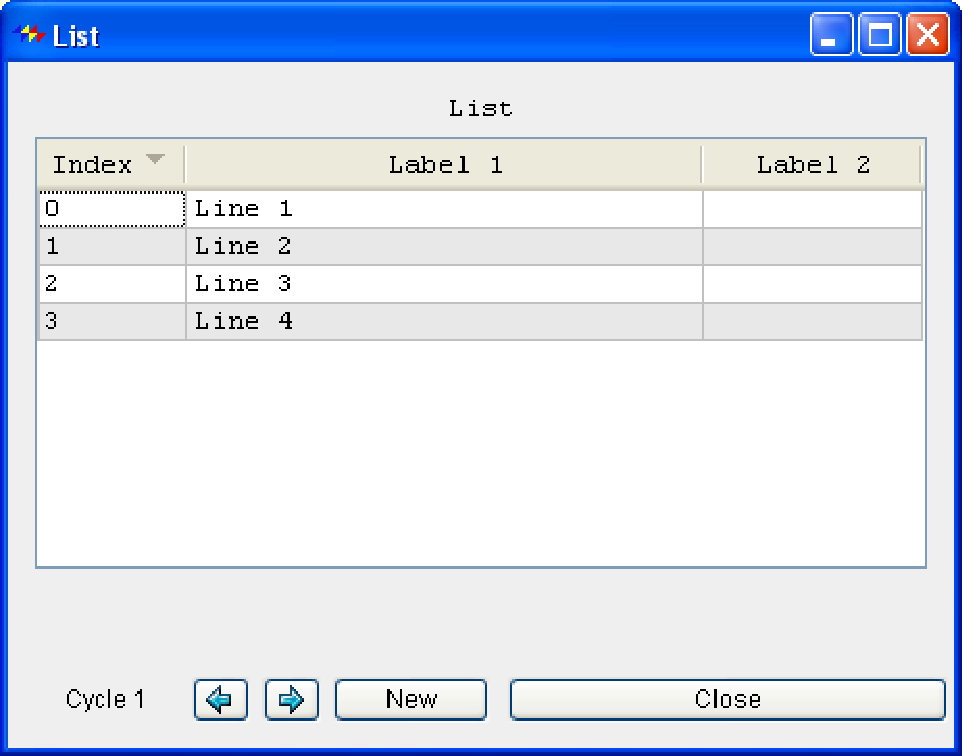
\includegraphics[width=0.6\linewidth]{grab_list}
   \end{center}
\caption{example of List}
\end{figure}
